\documentclass[11pt]{article}
\usepackage[margin=1in]{geometry}
\usepackage{amsmath,amssymb}
\usepackage{graphicx}
\usepackage{xcolor}
\usepackage{tikz}
\usetikzlibrary{decorations.pathreplacing,arrows.meta}
\usepackage{pgfplots}
\pgfplotsset{compat=1.17}
\usepackage{tcolorbox}
\usepackage{array}
\usepackage{enumitem}
\usepackage{hyperref}

\graphicspath{{figures/}}

% Notation
\newcommand{\xs}{x_{\text{stim}}}
\newcommand{\xd}{x_{\text{dist}}}
\newcommand{\xp}{x_{\text{perc}}}
\newcommand{\dd}{\delta_{\text{dist}}}
\newcommand{\PSEuni}{\mathrm{PSE}_{\text{uni}}}
\newcommand{\PSEbi}{\mathrm{PSE}_{\text{bi}}}
\newcommand{\high}{\text{``high''}}
\newcommand{\low}{\text{``low''}}
\newcommand{\bvec}{\vec{\beta}}

\definecolor{unicol}{RGB}{0,120,230}
\definecolor{bicol}{RGB}{205,0,0}

% Side remarks and questions from the handwritten notes
\newtcolorbox{aside}{colback=violet!4,colframe=violet!60!black,boxrule=0.5pt,
  left=4pt,right=4pt,top=2pt,bottom=2pt,fontupper=\small,
  title={\small Note},fonttitle=\bfseries\small,coltitle=white}
\newtcolorbox{result}{colback=green!6,colframe=green!45!black,boxrule=0.6pt}

\title{Perceptual Interpretation of Models}
\author{Vera Schroeder}
\date{November 2026\\[4pt]\small(typeset from handwritten notes for reference)}

\begin{document}
\maketitle
\tableofcontents
\newpage

%=====================================================================
\section{The psychometric function with lapses}

\begin{align*}
  P(\text{response} = \high) = P(r = 1)
  &= \psi(\xs; \bvec, \gamma_h, \gamma_\ell)\\
  &= \gamma_h + (1-\gamma_h-\gamma_\ell)\,F(\xs; \bvec),\\
  F(\xs; \bvec) &= \bigl[1+\exp\bigl(-(\beta_0+\beta_1\xs)\bigr)\bigr]^{-1}.
\end{align*}
The stimulus is normalized:
\[
  \mu_{\text{stim}} = 28, \qquad
  \sigma_{\text{stim}} = \operatorname{std}\{6,\dots,50\} \;(=14.63), \qquad
  \xs = \frac{\text{stim} - 28}{\sigma_{\text{stim}}}.
\]

$\gamma_h$ and $\gamma_\ell$ describe upper and lower bounds/asymptotes on the sigmoid
curve, but they can also be interpreted using a hidden-state mixture model:
\[
  P(\text{lapsed}) = \gamma_h + \gamma_\ell, \qquad
  P(\text{engaged}) = 1 - (\gamma_h + \gamma_\ell),
\]
\[
  P(r = 1 \mid \xs) =
  \begin{cases}
    \dfrac{\gamma_h}{\gamma_h+\gamma_\ell}, & \text{lapsed},\\[10pt]
    F(\xs; \bvec), & \text{engaged}.
  \end{cases}
\]
Now we put aside the lapses and focus only on the engaged state, with response
probability defined by $F$.

%=====================================================================
\section{Interpreting $F$ in terms of perception}

\[
  \xp = \xs + \varepsilon, \qquad \varepsilon \sim \operatorname{Logistic}[\mu, s],
  \qquad
  \mathbb{E}[\varepsilon] = \mu, \qquad \operatorname{Var}[\varepsilon] = \frac{s^2\pi^2}{3}.
\]

\begin{aside}
The noise distribution determines the type of sigmoid function. The logistic is
easier to work with algebraically than the normal; it has heavier tails.
\end{aside}

\begin{center}
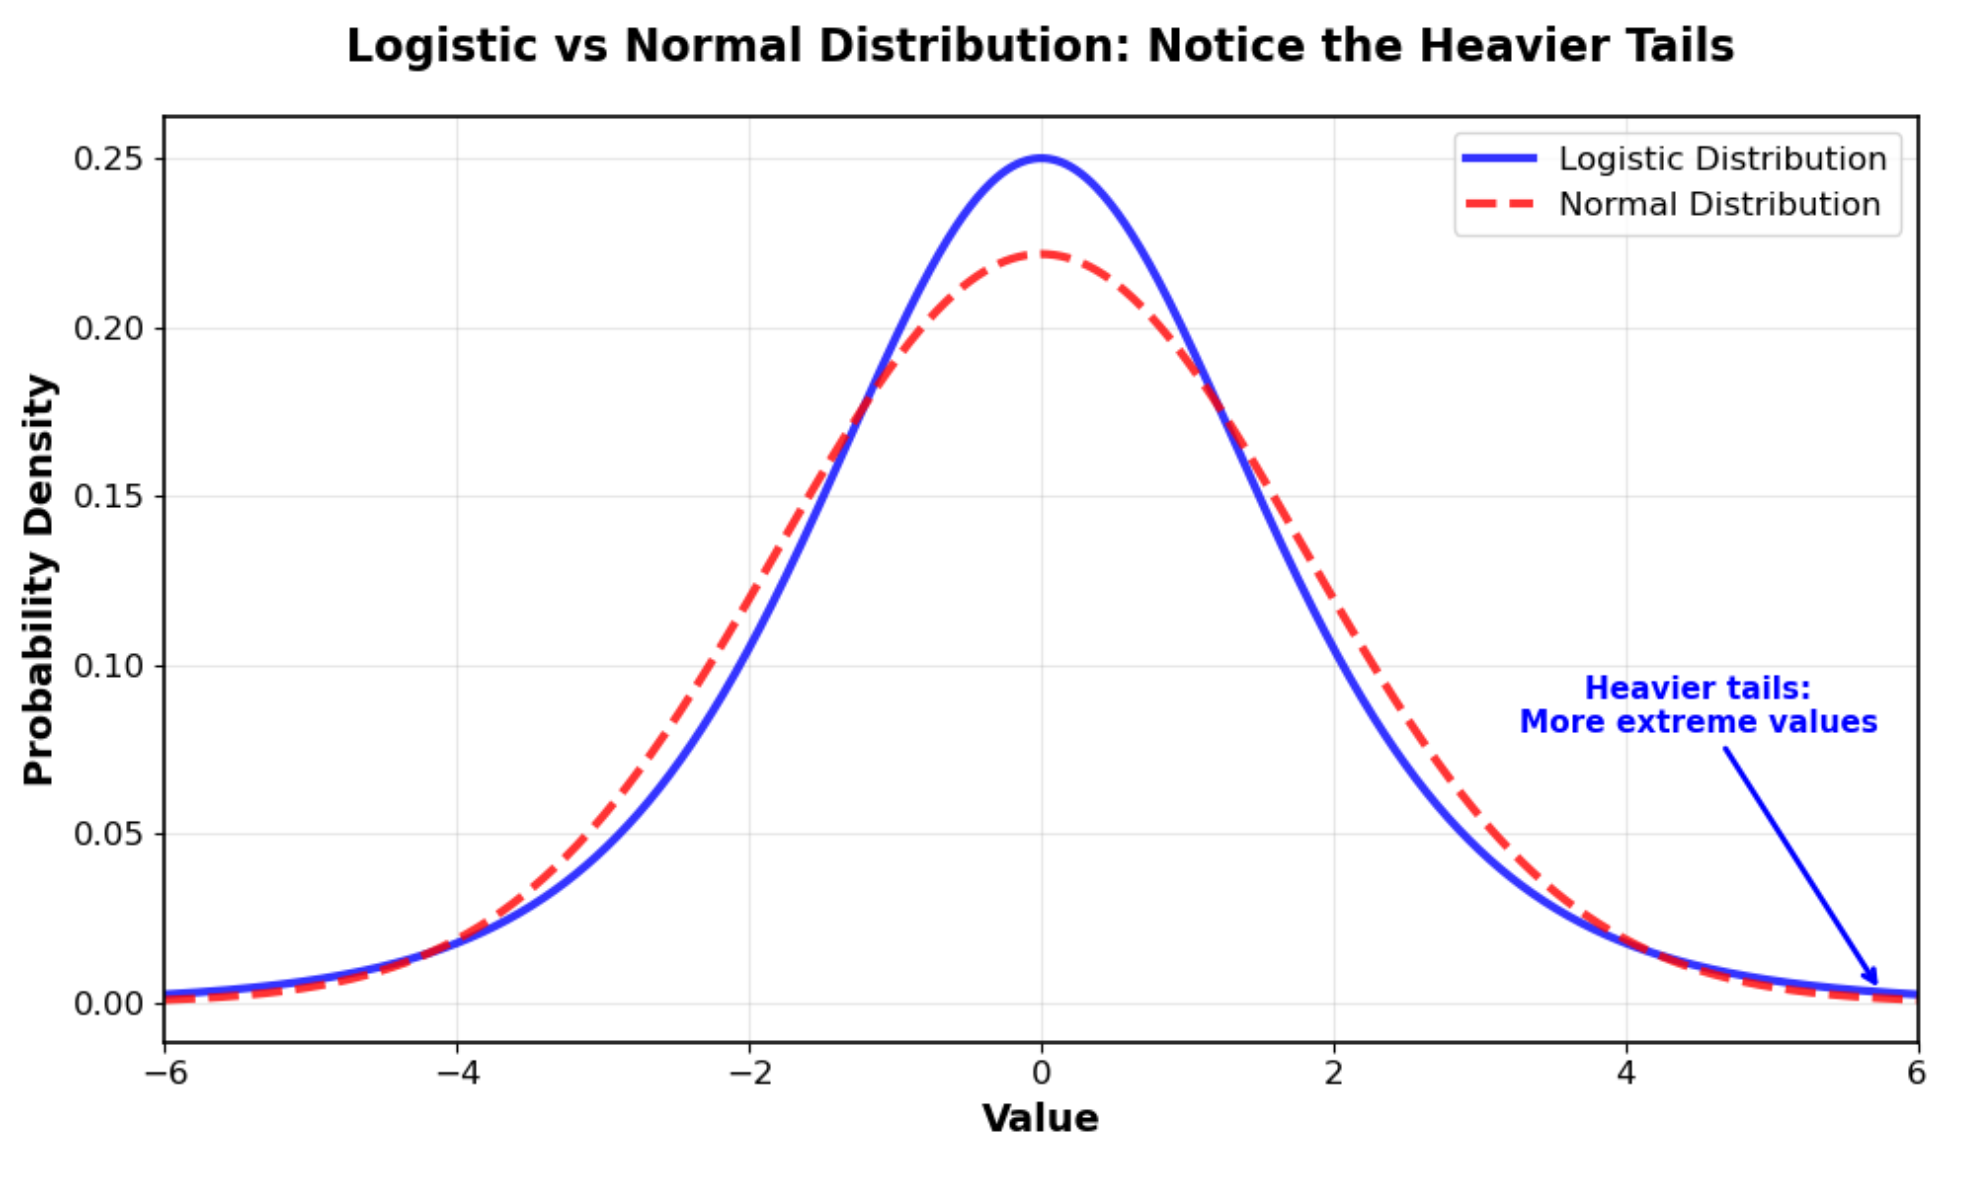
\includegraphics[width=0.6\textwidth]{logistic_vs_normal.png}
\end{center}

Let the decision rule on $\xp$ be
\[
  \text{response} =
  \begin{cases}
    \high, & \text{if } \xp > t,\\
    \low,  & \text{if } \xp < t.
  \end{cases}
\]
Now consider
\begin{align*}
  P(\text{response} = \high \mid \xs)
  &= P(\xp > t \mid \xs = x_s)\\
  &= P(\xs + \varepsilon > t \mid \xs = x_s)\\
  &= P(\varepsilon > t - x_s)\\
  &= 1 - P(\varepsilon < t - x_s)\\
  &= 1 - \frac{1}{1+\exp\Bigl[-\Bigl(\dfrac{(t-x_s)-\mu}{s}\Bigr)\Bigr]}\\
  &= \frac{1}{1+\exp\Bigl[\dfrac{t-x_s-\mu}{s}\Bigr]}
   = \frac{1}{1+\exp\Bigl[-\Bigl(\dfrac{\mu-t}{s}+\dfrac{1}{s}x_s\Bigr)\Bigr]}\\
  &= \frac{1}{1+\exp\bigl[-(\beta_0+\beta_1 x_s)\bigr]}
   = F\Bigl(x_s;\ \beta_0 = \frac{\mu-t}{s},\ \beta_1 = \frac{1}{s}\Bigr).
\end{align*}
This is equivalent to the previous construction of $F$.

\subsection{Interpreting $\bvec$}

\begin{itemize}
  \item $\beta_1 = \dfrac{1}{s}$:
  \begin{itemize}[nosep]
    \item larger $\beta_1$ $\iff$ smaller $s$ $\iff$ the noise varies less;
    \item smaller $\beta_1$ $\iff$ larger $s$ $\iff$ the noise varies more.
  \end{itemize}
  \item $\beta_0 = \dfrac{\mu - t}{s} = (\mu - t)\,\beta_1$, so $\dfrac{\beta_0}{\beta_1}$ indicates bias.
\end{itemize}

%=====================================================================
\section{How does this relate to the models I've been fitting?}

\paragraph{Model A} fits left/right $\times$ unimanual/bimanual separately. It assumes
the parameters $\gamma_h, \gamma_\ell, \beta_0, \beta_1$ are independent for each group.
\begin{aside}
Do the noise and lapse conditions differ
\begin{itemize}[nosep]
  \item between hands?
  \item between unimanual and bimanual cases?
\end{itemize}
\end{aside}

\paragraph{Model B} fits left/right $\times$ unimanual/bimanual separately. For each
group (assumed independent):
\begin{itemize}[nosep]
  \item assume the parameters $(\gamma_h, \gamma_\ell, \beta_0, \beta_1)$ vary between sessions;
  \item assume each session-level parameter comes from a shared group-level distribution;
  \item estimate each session-level parameter;
  \item estimate the group-level distributions' hyperparameters.
\end{itemize}
\begin{aside}
Do the noise and lapse conditions differ
\begin{itemize}[nosep]
  \item between hands?
  \item between unimanual and bimanual cases?
  \item between sessions?
\end{itemize}
\end{aside}

None of this explains the ``curve repulsion'' behavior we have observed. It suggests
the unimanual and bimanual cases might not be independent. So we bring the
distractor into the model.

%=====================================================================
\section{Model C: the distractor as a covariate}

\[
  F(\xs; \bvec) = \bigl[1+\exp\bigl(-(\beta_0+\beta_1\xs+\beta_2\xd)\bigr)\bigr]^{-1}
\]
For a model of bimanual interactions, consider
\[
  \xp = \xs + c\,\xd + \varepsilon, \qquad \varepsilon \sim \operatorname{Logistic}[\mu,s],
\]
with the same decision rule on $\xp$ ($\high$ if $\xp > t$, $\low$ if $\xp < t$).
Now consider
\begin{align*}
  P(\text{response} = \high \mid \xs, \xd)
  &= P(\xp > t \mid \xs = x_s,\ \xd = x_d)\\
  &= P(x_s + c x_d + \varepsilon > t)\\
  &= P(\varepsilon > t - x_s - c x_d)\\
  &= 1 - P(\varepsilon < t - x_s - c x_d)\\
  &= 1 - \frac{1}{1+\exp\Bigl[-\Bigl(\dfrac{(t-x_s-c x_d)-\mu}{s}\Bigr)\Bigr]}\\
  &= \frac{1}{1+\exp\Bigl[\dfrac{t-x_s-c x_d-\mu}{s}\Bigr]}\\
  &= \frac{1}{1+\exp\Bigl[-\Bigl(\dfrac{\mu-t}{s}+\dfrac{1}{s}x_s+\dfrac{c}{s}x_d\Bigr)\Bigr]}\\
  &= \frac{1}{1+\exp\bigl[-(\beta_0+\beta_1 x_s+\beta_2 x_d)\bigr]}\\
  &= F\Bigl(x_s;\ \beta_0 = \frac{\mu-t}{s},\ \beta_1 = \frac{1}{s},\ \beta_2 = \frac{c}{s}\Bigr).
\end{align*}

\subsection*{At what value of $\xs$ are responses \high{} and \low{} equally likely?}

\begin{itemize}
  \item \textbf{Unimanual trials} ($\xd = 0$):
  \[
    \frac{t - x_s - c(0) - \mu}{s} = 0
    \quad\Longrightarrow\quad
    x_s = t-\mu = \PSEuni
  \]
  \item \textbf{Bimanual trials} ($\xd = x_d > 0$):
  \[
    \frac{t - x_s - c x_d - \mu}{s} = 0
    \quad\Longrightarrow\quad
    x_s = t-\mu-c x_d = \PSEbi
  \]
\end{itemize}
$t$ and $\mu$ are not mutually identifiable, so take $\mu = 0$.

\begin{aside}
Since the presence of the distractor increases $\xp$, picking a lower threshold $t$
could increase the expected reward.
\end{aside}

%=====================================================================
\section{What decision boundary $t$ maximizes reward/accuracy?}

Construct the function $R(t) = P[\text{correct} \mid \text{boundary} = t]$ over the
stimulus set
\[
  \vec{x} = [\,\underbrace{6,12,18,24}_{\text{``low''}},\ \underbrace{32,38,44,50}_{\text{``high''}}\,].
\]
What is $P(\text{correct} \mid t, \text{trial conditions})$? With $\mu = 0$,
\begin{align*}
  P(\xp > t \mid \xs = x_s,\ \xd = x_d) &= \frac{1}{1+\exp\bigl[\tfrac{1}{s}(t-x_s-c x_d)\bigr]},\\
  P(\xp < t \mid \xs = x_s,\ \xd = x_d) &= \frac{1}{1+\exp\bigl[-\tfrac{1}{s}(t-x_s-c x_d)\bigr]}.
\end{align*}
\begin{aside}
The logistic function $g(x) = \dfrac{1}{1+e^{-x}}$ has the property $g(-x) = 1-g(x)$.
\end{aside}

\noindent $P(\text{correct}\mid t, x_s, x_d)$:

\begin{center}
\renewcommand{\arraystretch}{2.2}
\begin{tabular}{>{\centering\arraybackslash}m{2.6cm}|>{\centering\arraybackslash}m{5.6cm}|>{\centering\arraybackslash}m{5.6cm}}
 & $x_s \le 28$\newline {\small($x_s = x_i$, $i\le 4$)} & $x_s \ge 28$\newline {\small($x_s = x_j$, $j > 4$)}\\
\hline
Unimanual\newline $x_d = 0$ &
$P(x_p < t \mid x_s = x_i, x_d = 0, t)$\newline
$=\dfrac{1}{1+\exp\bigl[-\frac{1}{s}(t-x_i)\bigr]}$ &
$P(x_p > t \mid x_s = x_j, x_d = 0, t)$\newline
$=\dfrac{1}{1+\exp\bigl[\frac{1}{s}(t-x_j)\bigr]}$\\[8pt]
\hline
Bimanual\newline $x_d = X_D$ &
$P(x_p < t \mid x_s = x_i, x_d = X_D, t)$\newline
$=\dfrac{1}{1+\exp\bigl[-\frac{1}{s}(t-x_i-cX_D)\bigr]}$ &
$P(x_p > t \mid x_s = x_j, x_d = X_D, t)$\newline
$=\dfrac{1}{1+\exp\bigl[\frac{1}{s}(t-x_j-cX_D)\bigr]}$
\end{tabular}
\end{center}

\subsection{Priors on trial states and the expected reward}

Define prior distributions on trial states:
\begin{align*}
  P(x_d = X_D) &:= Q = 1 - P(x_d = 0),\\
  P(x_s = x_i) &:= q_i \quad\text{for } i = 1,\dots,8 \qquad \Bigl(\textstyle\sum_{i=1}^{8} q_i = 1\Bigr).
\end{align*}
Then
\begin{align*}
  R(t) &= P(\text{correct}\mid t)
  = \sum_{x_d}\sum_{x_s} P(\text{correct}\mid t, x_s, x_d)\, P(x_s \,\&\, x_d)\\
  &= (1-Q)\left[\sum_{i=1}^{4}\frac{q_i}{1+\exp\bigl[-\frac{1}{s}(t-x_i)\bigr]}
     + \sum_{j=5}^{8}\frac{q_j}{1+\exp\bigl[\frac{1}{s}(t-x_j)\bigr]}\right]\\
  &\quad + Q\left[\sum_{i=1}^{4}\frac{q_i}{1+\exp\bigl[-\frac{1}{s}(t-x_i-cX_D)\bigr]}
     + \sum_{j=5}^{8}\frac{q_j}{1+\exp\bigl[\frac{1}{s}(t-x_j-cX_D)\bigr]}\right].
\end{align*}

Find $t^*$ that maximizes $R(t)$ (in terms of all other parameters)\,---\,yikes!
Suppose instead that all trial states have equal prior probability:
$q_i = \tfrac18$ for $i = 1,\dots,8$, and $Q = \tfrac12$. Then
\begin{align*}
  R(t) = \frac{1}{16}\Biggl[
   &\sum_{i=1}^{4}\frac{1}{1+\exp\bigl[-\frac{1}{s}(t-x_i)\bigr]}
   + \sum_{j=5}^{8}\frac{1}{1+\exp\bigl[\frac{1}{s}(t-x_j)\bigr]}\\
   +&\sum_{i=1}^{4}\frac{1}{1+\exp\bigl[-\frac{1}{s}(t-x_i-cX_D)\bigr]}
   + \sum_{j=5}^{8}\frac{1}{1+\exp\bigl[\frac{1}{s}(t-x_j-cX_D)\bigr]}\Biggr].
\end{align*}

\begin{result}
Numerically, found
\(\displaystyle t^* \approx 28 + \tfrac12 c X_D\)
\quad(needs to be verified).
\end{result}

%=====================================================================
\section{What is the impact of $t^*$ on the PSEs?}

Recall: $\PSEuni = t$ and $\PSEbi = t - cX_D$ (with $\mu = 0$). With $t = t^*$,
\begin{align*}
  \color{unicol}\PSEuni^* &= 28 + \tfrac12 cX_D, &
  \color{bicol}\PSEbi^* &= 28 + \tfrac12 cX_D - cX_D = 28 - \tfrac12 cX_D.
\end{align*}
Therefore, a threshold on $\xp$ of $t = 28 + \frac12 cX_D$ yields
\[
  {\color{bicol}\PSEbi} < 28 < {\color{unicol}\PSEuni},
  \qquad\text{with}\qquad
  {\color{unicol}\PSEuni} - {\color{bicol}\PSEbi} = c X_D .
\]

\begin{center}
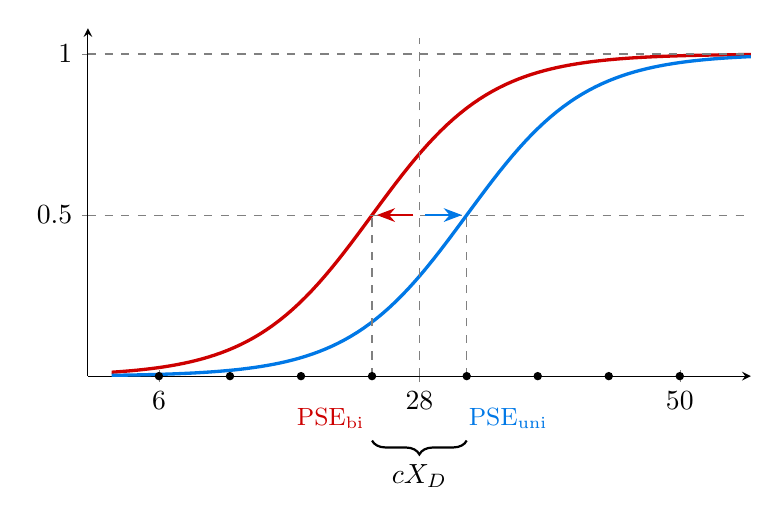
\begin{tikzpicture}
\begin{axis}[width=10cm,height=6cm,
  xmin=0,xmax=56,ymin=0,ymax=1.08,
  xtick={6,28,50},ytick={0.5,1},
  axis lines=left,clip=false]
  \addplot[domain=2:56,samples=100,very thick,bicol]{1/(1+exp(-(x-24)/5))};
  \addplot[domain=2:56,samples=100,very thick,unicol]{1/(1+exp(-(x-32)/5))};
  \addplot[only marks,mark=*,mark size=1.3pt] coordinates{(6,0)(12,0)(18,0)(24,0)(32,0)(38,0)(44,0)(50,0)};
  \draw[dashed,gray] (axis cs:0,1) -- (axis cs:56,1);
  \draw[dashed,gray] (axis cs:0,0.5) -- (axis cs:56,0.5);
  \draw[dashed,gray] (axis cs:28,0) -- (axis cs:28,1.05);
  \draw[dashed,gray] (axis cs:24,0) -- (axis cs:24,0.5);
  \draw[dashed,gray] (axis cs:32,0) -- (axis cs:32,0.5);
  \draw[-{Stealth},thick,bicol] (axis cs:27.5,0.5) -- (axis cs:24.4,0.5);
  \draw[-{Stealth},thick,unicol] (axis cs:28.5,0.5) -- (axis cs:31.6,0.5);
  \node[bicol,font=\small,anchor=north] at (axis cs:20.5,-0.07) {$\PSEbi$};
  \node[unicol,font=\small,anchor=north] at (axis cs:35.5,-0.07) {$\PSEuni$};
  \draw[decorate,decoration={brace,mirror,amplitude=5pt},thick]
    (axis cs:24,-0.2) -- (axis cs:32,-0.2) node[midway,below=5pt] {$cX_D$};
\end{axis}
\end{tikzpicture}
\end{center}

So Model C is theoretically consistent with this repulsion behavior. Let's talk details.

\subsection{Model C: structure and key assumptions}

Model C fits left/right separately. For each hand (assumed independent):
\begin{itemize}[nosep]
  \item assume the parameters $(\gamma_h, \gamma_\ell, \beta_0, \beta_1, \beta_2)$ vary between sessions;
  \item assume each session-level parameter comes from a shared hand-level distribution;
  \item estimate each session-level parameter;
  \item estimate the hand-level distributions' hyperparameters.
\end{itemize}
\begin{aside}
Do the noise conditions, lapses, and distractor-induced biases differ
\begin{itemize}[nosep]
  \item between hands?
  \item between unimanual and bimanual cases?
  \item between sessions?
\end{itemize}
\end{aside}

\paragraph{Key assumptions} (with $\xp = \xs + c\,\xd + \varepsilon$):
\begin{itemize}[nosep]
  \item the distractor impacts perception bias but not noise;
  \item the distractor's bias impact is linear in its strength;
  \item the hands' effects are separate;
  \item all parameters vary between sessions.
\end{itemize}

%=====================================================================
\section{Next: Model D}

\[
  F(\xs; \bvec) = \bigl[1+\exp\bigl(-(\beta_0+\beta_1\xs+\beta_2\xd+\beta_3\dd)\bigr)\bigr]^{-1},
  \qquad
  \dd =
  \begin{cases}
    0, & \text{unimanual trials},\\
    1, & \text{bimanual trials},
  \end{cases}
\]
where $\dd$ is the distractor indicator. For a model of bimanual interactions, consider
\[
  \xp = \xs + \varepsilon + \underbrace{b\,\dd + c\,\xd}_{=\,0 \text{ for unimanual trials}},
  \qquad \varepsilon \sim \operatorname{Logistic}[\mu,s],
\]
with the same decision rule on $\xp$. Now consider
\begin{align*}
  P(\text{response} = \high \mid \xs, \xd, \dd)
  &= P(\xp > t \mid \xs = x_s,\ \xd = x_d,\ \dd = \delta_d)\\
  &= P(x_s + c x_d + \varepsilon + b\,\delta_d > t)\\
  &= P(\varepsilon > t - x_s - c x_d - b\,\delta_d)\\
  &= 1 - P(\varepsilon < t - x_s - c x_d - b\,\delta_d)\\
  &= \frac{1}{1+\exp\Bigl[-\Bigl(\dfrac{\mu-t}{s}+\dfrac{1}{s}x_s+\dfrac{c}{s}x_d+\dfrac{b}{s}\delta_d\Bigr)\Bigr]}\\
  &= \frac{1}{1+\exp\bigl[-(\beta_0+\beta_1 x_s+\beta_2 x_d+\beta_3\delta_d)\bigr]}\\
  &= F\Bigl(x_s;\ \beta_0 = \frac{\mu-t}{s},\ \beta_1 = \frac{1}{s},\ \beta_2 = \frac{c}{s},\ \beta_3 = \frac{b}{s}\Bigr).
\end{align*}

\subsection{Model D: parameters and assumptions}

\[
  \psi = \gamma_h + (1-\gamma_h-\gamma_\ell)\,
  \frac{1}{1+\exp\bigl(-[\beta_0+\beta_1\xs+\beta_2\xd+\beta_3\dd]\bigr)}
\]

\begin{center}
\renewcommand{\arraystretch}{1.3}
\begin{tabular}{c|c|c|c}
Parameter & per hand & per uni/bi & per session\\
\hline
$\gamma_h$     & \checkmark & \checkmark & \\
$\gamma_\ell$  & \checkmark & \checkmark & \\
$\beta_0$      & \checkmark &            & \checkmark\\
$\beta_1$      & \checkmark &            & \checkmark\\
$\beta_2$      & \checkmark &            & \\
$\beta_3$      & \checkmark &            & \\
\end{tabular}
\end{center}

\paragraph{Assumptions:}
\begin{itemize}[nosep]
  \item lapse rates may differ between uni/bi trials, but don't differ between sessions;
  \item noise may differ between sessions, but doesn't differ between uni/bi trials;
  \item distractor-related bias varies with distractor strength, but not with session;
  \item distractor presence alone may be associated with bias.
\end{itemize}

\subsection*{To analyze next}
\begin{itemize}[nosep]
  \item Relate D to the decision rule and curve repulsion.
  \item Design a model consistent with noise variance changing with the distractor.
\end{itemize}

\end{document}
